\begin{figure}[!ht]
  \centering
  \begin{subfigure}[t]{0.3\textwidth}
    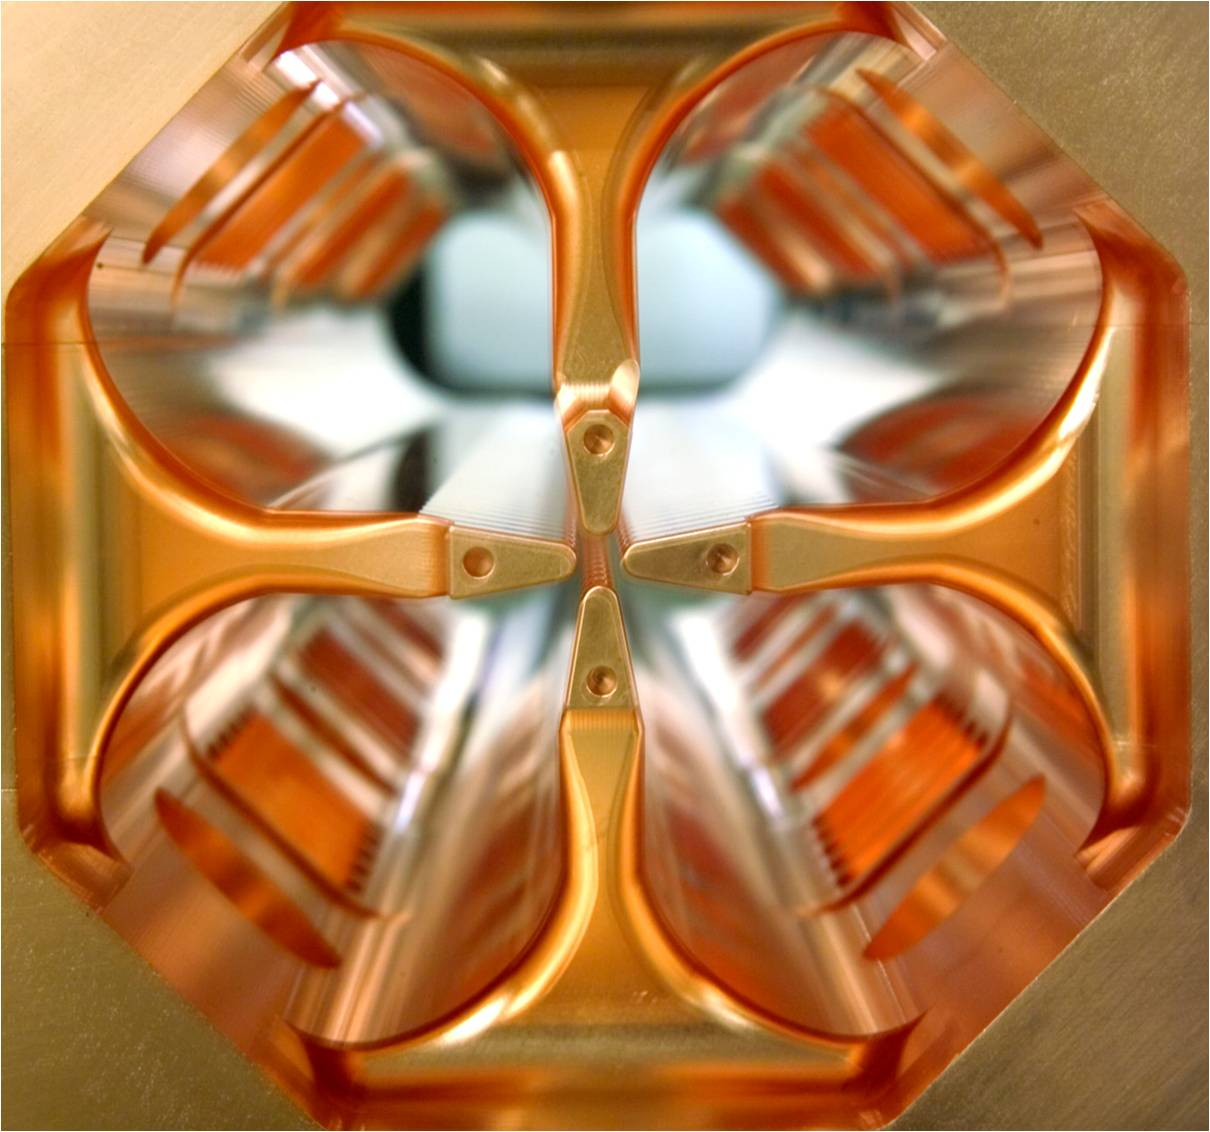
\includegraphics[width=\textwidth]{02_BeamDiag/figures/fig000_RFQ_c}
    \caption[The four copper vanes of a RFQ]{The four copper vanes (poles) of a RFQ.}
    \label{chap2:fig:RFQ_c}
  \end{subfigure}
  ~
  \begin{subfigure}[t]{.3\textwidth}
    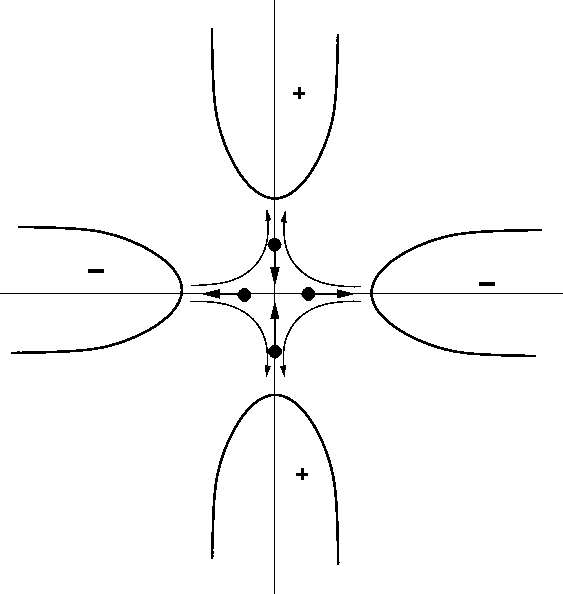
\includegraphics[width=\textwidth]{02_BeamDiag/figures/fig000_RFQ_a}
    \caption{Cut view of the transverse field.}
    \label{chap2:fig:RFQ_a}
  \end{subfigure}
  ~
  \begin{subfigure}[t]{0.3\textwidth}
    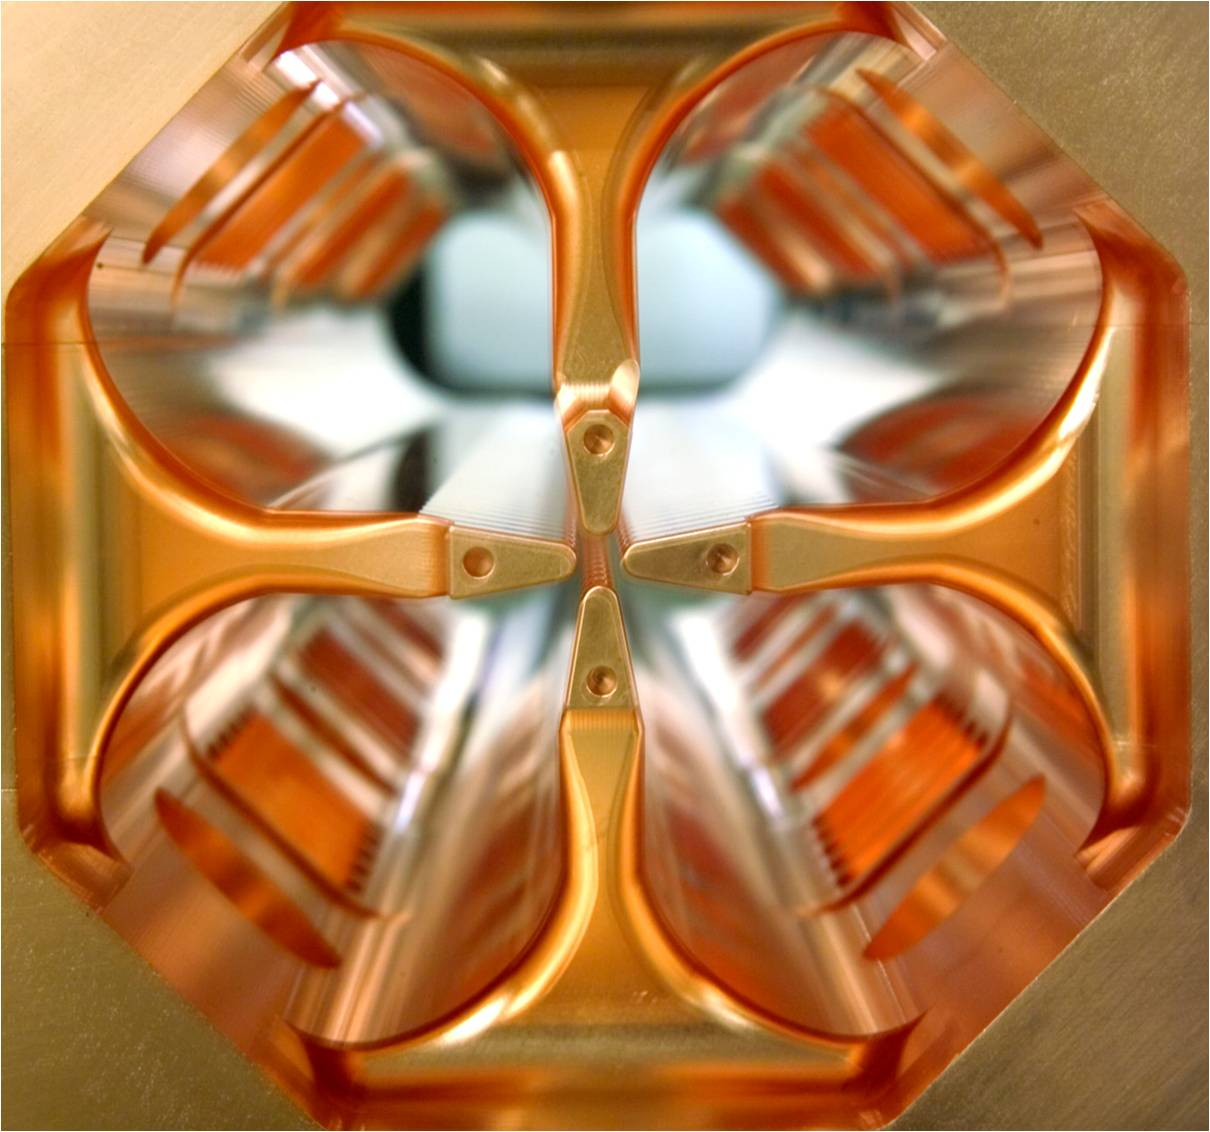
\includegraphics[width=\textwidth]{02_BeamDiag/figures/fig000_RFQ_b}
    \caption[Longitudinal modulation leading to an accelerating field]{Longitudinal modulation leading to an accelerating field \cite{Lombardi:1005049}.}
    \label{chap2:fig:RFQ_b}
  \end{subfigure}

  \caption[An RFQ structure bunches, focuses and accelerates charged particles by means of four poles that modulate the RF wave.]{An RFQ structure bunches, focuses and accelerates charged particles by means of four poles that modulate the RF wave.}
  \label{chap2:fig:RFQ}
\end{figure}
